\documentclass{article}
\usepackage[utf8]{inputenc}

\title{Relatório - Atividade 2, SCC0902}
\author{
  Marco Antônio Ribeiro de Toledo, RA: 11796419 \\
  Vítor Beneti Martins, RA: 11877635 \\
  Jayro Boy V. Neto, RA: 9762880 \\
  Lucas Massao Fukusawa Dagnone, RA: 11295810
}
\date{Junho de 2021}

\usepackage{natbib}
\usepackage{graphicx}
\usepackage{amsmath}
\usepackage{amssymb}
\usepackage{float}

\begin{document}

\maketitle

\tableofcontents
\listoffigures

\section{Testes de entrada binária}

\begin{figure}[H]
  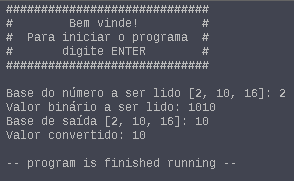
\includegraphics[width=\linewidth]{./CasoBin1}
  \caption{Entrada: 1010, saída decimal}
  \label{fig:bin1}
\end{figure}

\begin{figure}[H]
  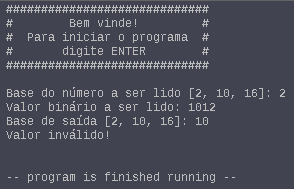
\includegraphics[width=\linewidth]{./CasoBin2}
  \caption{Entrada: 1012, saída decimal}
  \label{fig:bin2}
\end{figure}

\begin{figure}[H]
  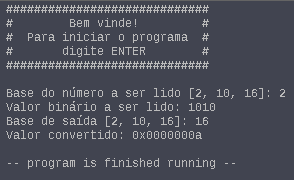
\includegraphics[width=\linewidth]{./CasoBin3}
  \caption{Entrada: 1010, saída hexadecimal}
  \label{fig:bin3}
\end{figure}

\begin{figure}[H]
  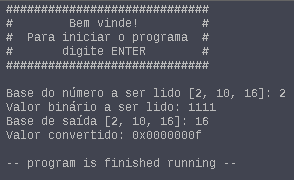
\includegraphics[width=\linewidth]{./CasoBin4}
  \caption{Entrada: 1111, saída hexadecimal}
  \label{fig:bin4}
\end{figure}

\begin{figure}[H]
  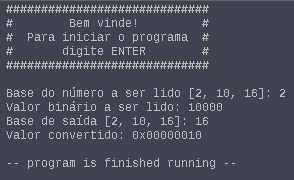
\includegraphics[width=\linewidth]{./CasoBin5}
  \caption{Entrada: 10000, saída hexadecimal}
  \label{fig:bin5}
\end{figure}

\begin{figure}[H]
  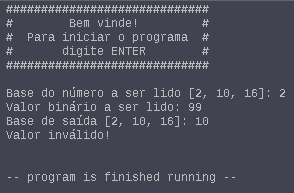
\includegraphics[width=\linewidth]{./CasoBin6}
  \caption{Entrada: 99, saída decimal}
  \label{fig:bin6}
\end{figure}

\begin{figure}[H]
  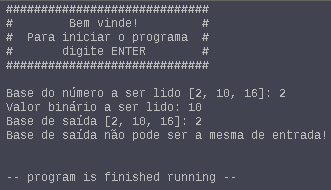
\includegraphics[width=\linewidth]{./CasoBin7}
  \caption{Entrada: 10, saída binária}
  \label{fig:bin7}
\end{figure}

\begin{figure}[H]
  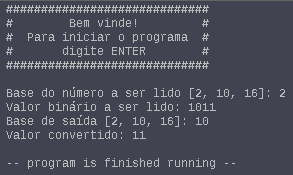
\includegraphics[width=\linewidth]{./CasoBin8}
  \caption{Entrada: 1011, saída decimal}
  \label{fig:bin8}
\end{figure}

\section{Testes de entrada decimal}

\begin{figure}[H]
  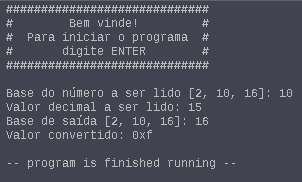
\includegraphics[width=\linewidth]{./CasoDec1}
  \caption{Entrada: 15, saída hexadecimal}
  \label{fig:dec1}
\end{figure}

\begin{figure}[H]
  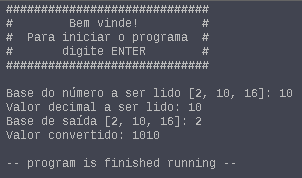
\includegraphics[width=\linewidth]{./CasoDec2}
  \caption{Entrada: 10, saída binária}
  \label{fig:dec2}
\end{figure}

\begin{figure}[H]
  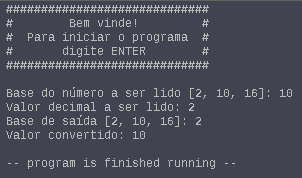
\includegraphics[width=\linewidth]{./CasoDec3}
  \caption{Entrada: 2, saída binária}
  \label{fig:dec3}
\end{figure}

\begin{figure}[H]
  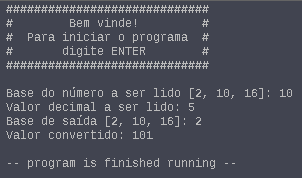
\includegraphics[width=\linewidth]{./CasoDec4}
  \caption{Entrada: 5, saída binária}
  \label{fig:dec5}
\end{figure}

\begin{figure}[H]
  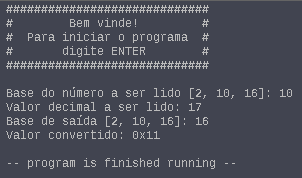
\includegraphics[width=\linewidth]{./CasoDec5}
  \caption{Entrada: 17, saída hexadecimal}
  \label{fig:dec5}
\end{figure}

\begin{figure}[H]
  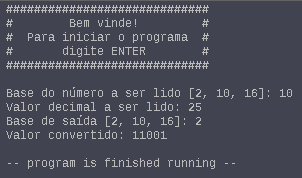
\includegraphics[width=\linewidth]{./CasoDec6}
  \caption{Entrada: 25, saída binária}
  \label{fig:dec6}
\end{figure}

\begin{figure}[H]
  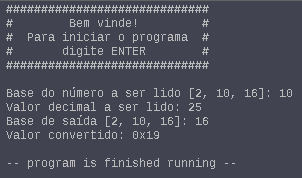
\includegraphics[width=\linewidth]{./CasoDec7}
  \caption{Entrada: 25, saída hexadecimal}
  \label{fig:dec7}
\end{figure}

\begin{figure}[H]
  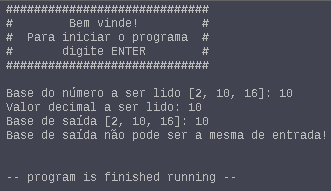
\includegraphics[width=\linewidth]{./CasoDec8}
  \caption{Entrada: 10, saída decimal}
  \label{fig:dec8}
\end{figure}

\section{Testes de entrada hexadecimal}

\begin{figure}[H]
  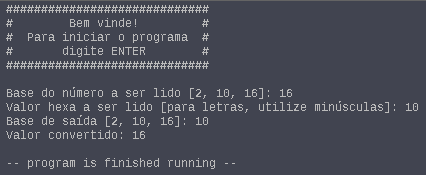
\includegraphics[width=\linewidth]{./CasoHexa1}
  \caption{Entrada: 10, saída decimal}
  \label{fig:hexa1}
\end{figure}

\begin{figure}[H]
  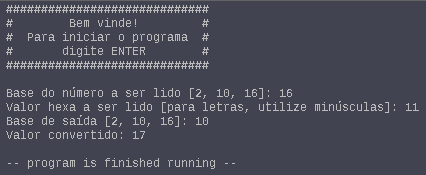
\includegraphics[width=\linewidth]{./CasoHexa2}
  \caption{Entrada: 11, saída decimal}
  \label{fig:hexa2}
\end{figure}

\begin{figure}[H]
  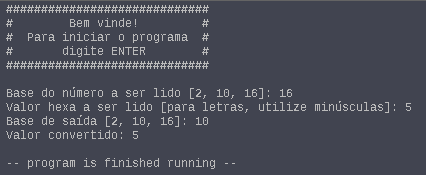
\includegraphics[width=\linewidth]{./CasoHexa3}
  \caption{Entrada: 5, saída decimal}
  \label{fig:hexa3}
\end{figure}

\begin{figure}[H]
  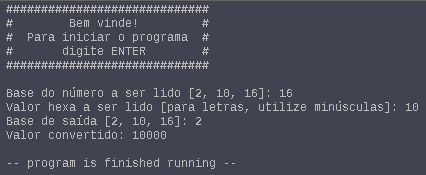
\includegraphics[width=\linewidth]{./CasoHexa4}
  \caption{Entrada: 10, saída binária}
  \label{fig:hexa5}
\end{figure}

\begin{figure}[H]
  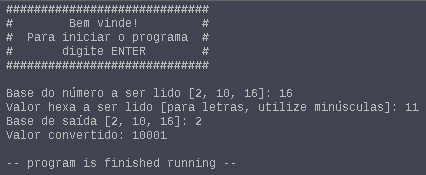
\includegraphics[width=\linewidth]{./CasoHexa5}
  \caption{Entrada: 11, saída binária}
  \label{fig:hexa5}
\end{figure}

\begin{figure}[H]
  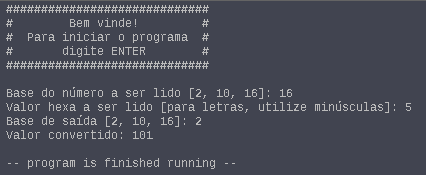
\includegraphics[width=\linewidth]{./CasoHexa6}
  \caption{Entrada: 5, saída binária}
  \label{fig:hexa6}
\end{figure}

\begin{figure}[H]
  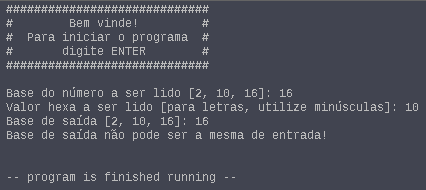
\includegraphics[width=\linewidth]{./CasoHexa7}
  \caption{Entrada: 10, saída hexadecimal}
  \label{fig:hexa7}
\end{figure}

\begin{figure}[H]
  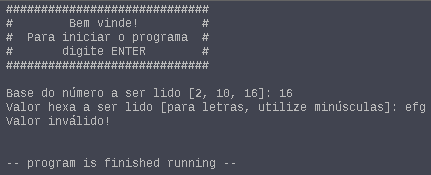
\includegraphics[width=\linewidth]{./CasoHexa8}
  \caption{Entrada: `efg`}
  \label{fig:hexa8}
\end{figure}

\section{Tratamento de erro de entrada}

\begin{figure}[H]
  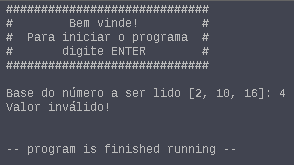
\includegraphics[width=\linewidth]{./CasoErro1}
  \caption{Base 4}
  \label{fig:erro1}
\end{figure}

\begin{figure}[H]
  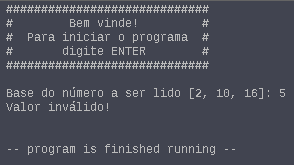
\includegraphics[width=\linewidth]{./CasoErro2}
  \caption{Base 5}
  \label{fig:erro2}
\end{figure}

\end{document}
